% !TEX root = ../main.tex

\chapter{顶层架构和模块}
这一章将详细阐述芯片的顶层架构设计和深度学习加速器模块与架构的逻辑关系设计。
在进行架构设计和具体的模块设计之前,先对需求进行分析和总结。
每个小节都将详细阐述所设计的模块和对设计内容建模,来实现和验证在CIS芯片上的基于脉动阵列的ResNet18硬件加速运算。


\section{顶层架构设计}
这一小节将描述芯片的顶层架构设计。
CIS的顶层架构设计是由CPU、高速总线、存储以及数据通路上的各个外设组成。
在后续的讨论中,将会把CPU、高速总线、存储器等基础组件做为设计内容中的一些设定。
本文将假设输入到深度学习运算模块的数据流,是一种理想的图像数据。
对于CIS上深度学习运算模块的设计,我们可以参考ISP芯片的设计逻辑。
因为我们可以将深度学习运算模块也视作一种图像处理的模块。  

\paragraph{系统需求}
整个设计的过程将采取自顶向下的策略。
首先设计CIS芯片的系统架构。
CIS芯片的系统架构包括了CPU、总线、ROM、SRAM、DRAM以及图像数据信号通路上的各个模块。
CPU和总线是芯片上必不可少的设备。
CPU能够执行程序和处理外设发出的中断。
总线是芯片上各个功能部件之间信息传输的干线。
这里设计的总线协议为AHB总线协议。
这是一种在嵌入式设备上非常常见的总线协议。
AHB总线是由主机、从机和其他基础设施构成的。
基础设施中包含了仲裁器、数据的多路选择器、地址的多路选择器、译码器。
这里的CPU和总线等基本设备在SoC的作用主要有以下几点:
% 1. 作为bootloader的控制器和基础设施;
% 2. 用于支持SoC业务的控制逻辑;
% 3. 用于响应外设的中断信号;
% 4. 搬运一些没有使用DMA的数据;
\begin{enumerate}
    \item 作为bootloader的控制器和基础设施;
    \item 用于支持SoC业务的控制逻辑;
    \item 用于响应外设的中断信号;
    \item 搬运一些没有使用DMA的数据;
\end{enumerate}    

本课题中的深度学习算法的运算将全部由专门的硬件加速部件来完成运算,因此下文将不再具体展开CPU和总线的类型和设计。
关于存储设备,课题中将讨论选用存储器的种类和不同种类存储器所需要的存储大小。
因为通常在一些小型的CIS中,芯片所需的内存很少,所以只需要选用SRAM就可以满足系统的需要。
在考虑到深度学习神经网络的模型的大小,同时也参考了一些业内的深度学习神经网络运算专用芯片,
本课题中的设计将同时使用SRAM和DRAM。
系统使用DRAM来存储模型的数据。


\subsection{架构详细设计}
从图\ref{fig:top_arch}中可以看到,这是图像传感器与ISP以及其他功能部件连接在一条高速数据总线的结构。
总体架构可以分为几个部分:数据通路部分、系统控制部分和高速数据总线。
数据通路部分包含了IDA(Input Data Adapter)、深度学习神经网络加速模块、TX输出模块。
系统控制部分包含了CPU、DMA、Memory、SPI Flash以及其他外设模块(比如$I^2C$和UART等接口模块)。
%TODO 架构图展示
\begin{figure}[htbp]
    \centering
    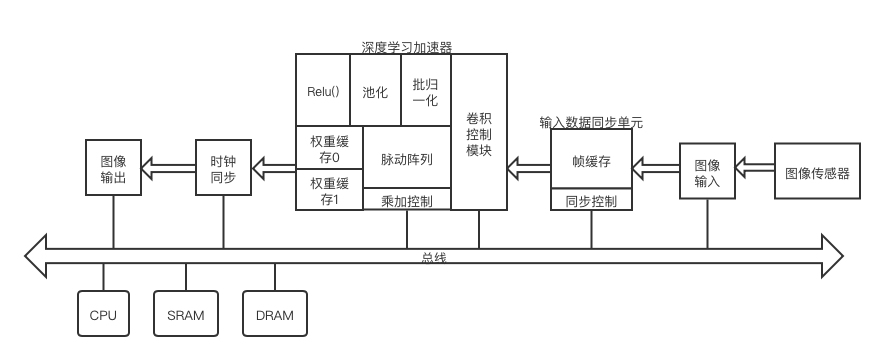
\includegraphics[width=15cm,height=6cm]{figures/top_arch.png}
    \caption{总体架构图}
    \label{fig:top_arch}
\end{figure}
%TODO 各个模块的简述
这里的视频数据格式为RGB888。
因此,我们可以轻松将其转化为深度学习加速器模块需要的输入数据尺寸224x224x3个像素点。


\subsection{顶层逻辑的建模}

基于systemc实现的顶层逻辑中,将实例化在第2小节中设计的各个模块,以及定义模块间的信号和控制逻辑。
同时,顶层逻辑将绑定各个模块之间的接口和信号。
最后,顶层逻辑将初始化仿真。
在本课题中,顶层逻辑将产生一个系统时钟信号,而图像数据将在数据输入同步单元中直接产生。  

在顶层架构中我们设计了一个“img_gen”模块来仿效传感器核心输出的图像数据信号。
这个模块将通过DVP接口向数据通路后端的模块输出图像。
接口主要包括了像素信号、行同步信号、帧同步信号,以及图像数据信号。


\begin{codeblock}[language=c++]
#include “systemc.h”
#include "img_gen.h"
#include "input_sync.h"
#include "systolic_top.h"

int sc_main(int, char *[])
{
  //Signals
  sc_signal<bool> src_pclk;
  sc_signal<bool> src_vsync;
  sc_signal<bool> src_hsync;
  sc_signal<sc_uint<11>> src_data;

  //Clock
  sc_signal<bool> clk;

  //Instance of 'img\_{}gen' module
  img_gen I("img_gen");
  //Positional port binding
  I(src_pclk, src_vsync, src_hsync, src_data, clk);

  //Instance of 'input\_{}sync' module
  input_sync IN("input_sync");
  //Named port binding
  IN.pclk(src_pclk)
  IN.vsync(src_vsync)
  IN.hsync(src_hsync)
  IN.data(src_data)
  //Positional port binding
  IN(sync_pclk, sync_vsync, sync_hsync, resized_data)

  //Instance of 'dl\_{}acc' module
  systolic_top S("systolic_top");
  //Named port binding
  S.pclk(sync_pclk);
  S.vsync(sync_vsync);
  S.hsync(sync_hsync);
  S.data(resized_data);

  //Initialize simulation
  sc_start(0, SC_NS);
  for(int i = 0; i < 224*224*3*8; i++){
    clk.write(1);
    sc_start(10, SC_NS);
    clk.write(0);
    sc_start(10, SC_NS);
  }

  return 0;
}

\end{codeblock}

下面是基于systemc定义了"img_gen"模块来仿效传感器输出的图像信号。
这里依赖了systemc提供的特性来模拟出模块根据系统时钟的频率进行工作。
stream_on()是一个model函数,它替代了产生图像的硬件行为。
每一个系统时钟频率的周期中,stream_on()函数都将按照一定的规则输出图像信号。
这里我们将通过配置来指定"img_gen"模块输出的图像信号所表达的每一帧图像的尺寸,以及输出时所用的像素频率、行同步信号的频率、帧的fps。

\begin{codeblock}[language=c++]
#include "systemc.h"

struct img_gen : sc_module{
  sc_out<bool>PCLK,VSYNC,HSYNC;
  sc_out<sc_uint<11>> DATA;
  sc_in<bool> XCLK;

  void stream_on(void);
  
  SC_CTOR(img_gen){
  SC_METHOD(stream_on):
    dont_initialize();
    sensitive << XCLK.pos();
  }
}

\end{codeblock}

\section{数据通路中的模块}
图像数据通路的设计是本课题的核心部分。
CIS芯片的基本需求就是将光学图像转换成电信号,再将电信号经过模拟信号转换为数字信号。
在CIS芯片将数据转换为数字信号后,它还会将数字信号进行处理,输出用户需求的图像信息。
这个信号从前向后传输并转换的逻辑像一条通道,因此称之为图像数据通路。

本课题要做的就是在CIS芯片进行数字信号处理时,增加硬件加速的深度学习神经网络推理运算。
本章将分别阐明数据流的输入,数据的运算,数据流的输出三个部分的所有模块设计原理。
其中,各小节会着重描述数据流的组件间逻辑关系,以及各个模块控制流的状态机和执行逻辑。

\subsection{模块需求}

一般的,在芯片中CPU用于执行固件的程序。
这些程序可以被用于初始化设备,或者与主机通信。
图像数据的处理过程是由数据通路中的每个模块完成的。
这个小节将分析每个模块的功能,以及模块间的数据流和控制流关系。
首先,我们可以分解需求并得到以下列出的需求点:
\begin{enumerate}
    \item 数据通路中的基本模块
    \item 脉动阵列的设计
    \item ResNet18在脉动阵列上的实现
\end{enumerate}    

\paragraph{数据通路}
图像数据通路是深度学习加速器的基础。
数据通路的基本功能就是数据的输入、数据的处理和数据的输出。
对于深度学习神经网络加速器,我们需要设计一个配合加速器工作的数据信号输入模块。
这个模块需要根据后文描述的加速器的行为,将视频数据流中的数据按照加速器所需的数据宽度、数据格式和频率放置到加速器的输入缓冲中。
神经网络加速器就是整个数据通路中用于深度学习神经网络运算的模块。
它需要满足ResNet18网络结构的所有运算。
加速器的具体设计将在下一个章节中详细描述。
在加速器完成基于ResNet18的图像识别运算之后,由图像输出时钟域中的模块缓存图像帧数据并向后通过CSI接口输出给主机。


CIS芯片的作用,就是将图像传感器接收到的信号,转为数字信号后传输给后端。
芯片上图像数字信号所经过的所有模块连接起来就像是一条单向的通道。
一般的,我们称这些模块所组成的通道为图像数据通路。
图像数据通路一般由输入、数据处理和输出三个部分组成。
通常地,这三个部分也具有各自不同的时钟域。

%TODO 架构图展示
\begin{figure}[htbp]
    \centering
    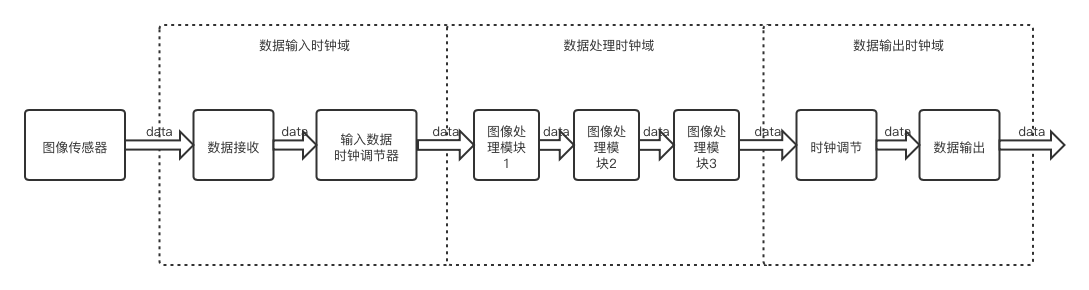
\includegraphics[width=15cm,height=5cm]{figures/datapath.png}
    \caption{图像信号处理的数据流图}
    \label{fig:datapath}
\end{figure}

%TODO 这里先描述以下datapath,包括DI、DP、DO三个时钟域。
如图\ref{fig:datapath}所示,图像处理部件的前后分别需要设置两个不同的时钟域用于输入和输出图像数据的信号。
因此,我们在设计CIS的数据通路中的深度学习运算模块时,也需要做相同的设计。
将输入模块的图像数据信号按一定的顺序排列好,按照脉动阵列的特性以一定的方式依次输入到阵列中。


在输入时钟域中,RX模块接收从CMOS传感器输出的数据。
由一个缓冲区暂存数据,经过时钟同步和一些预处理后向后面的数据处理时钟域输出数据。
在数据处理的时钟域中,深度学习运算模块将进行推理操作。
在输出时钟域中,FT(fix timing)模块将调整输出的时钟频率.TX模块负责以指定格式输出图像数据。  


% \subparagraph{脉动阵列}
% 在脉动阵列中,需要设计每个处理单元的逻辑和工作行为。
% 在实现神经网络算法时,需要分解出所有使用到的运算符,并分析哪些可以通过脉动阵列的乘加运算矩阵加速。


\subsection{模块设计}
图像数据通路的整体设计如图所示\ref{fig:image_datapath},在整个图像数据通路中有三个不同的时钟域。
\begin{figure}[htbp]
    \centering
    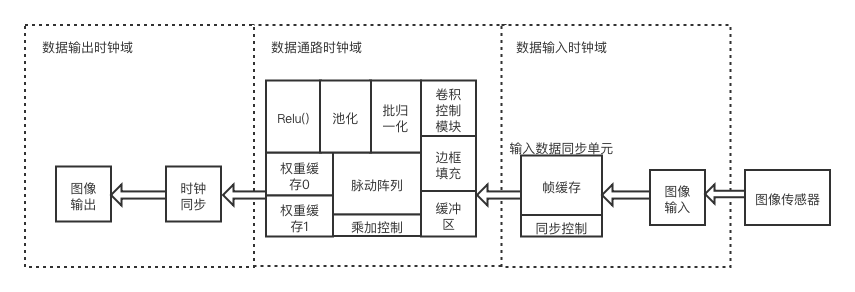
\includegraphics[width=15cm,height=6cm]{figures/image_datapath.png}
    \caption{图像数据通路架构图}
    \label{fig:image_datapath}
\end{figure}
区分这三个时钟域的目的是支持3个不同的时钟频率。
它们分别是图像传感器的输入数据信号的时钟、深度学习加速器的运行时钟和特征图的输出数据信号的时钟。
在这个数据通路中,最重要的模块就是深度学习运算加速器模块。


\paragraph{数据流的输入}
% TODO 
%   数据流的输入将由IDA(Input Data Adapter)模块处理。这个模块的主要作用是将Sensor输出的数据放到一个缓存区。
%   并将视频数据流的plck同步到数据流的时钟域。

这里假设从图像传感器输出的图像数据为224x224像素尺寸的图像。
视频数据流的输入需要参考流式设备的特性,合理的缓存大小和同步的时机是关键点。
对于卷积运算,缓存的行数大小应该大于等于卷积核的行数和列数之间的较大值。
例如,卷积核的尺寸为3x3时,缓存至少要保存3行数据。
如果,每帧图像的尺寸为224x224个像素点。
由RGB三个通道组成的每一帧都拆分成三个224x224x8比特流。
那么需要给一个通道的一帧数据缓存的大小需要大于等于672个字节。

\begin{figure}[htbp]
    \centering
    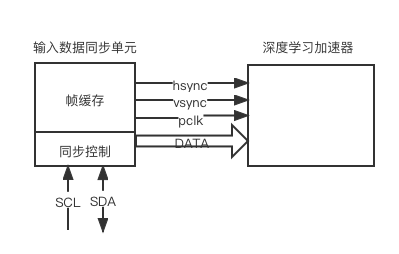
\includegraphics[width=12cm,height=8cm]{figures/input_data_adapter.png}
    \caption{输入数据同步单元架构图}
    \label{fig:input_data_adapter}
\end{figure}

如图\ref{fig:input_data_adapter}是数据输入同步单元与深度学习加速器之间的连线设计。
hsync用于行同步信号。
vsync用于帧同步信号。
pclk是像素时钟信号。
data是并行的图像数据,这里设定为8bit带宽。
SCL和SDA是用来读写模块寄存器的I2C接口的时钟信号和数据信号。


\paragraph{数据流中的运算}
% TODO
% 在数据流中实时运算图像识别的算法
深度学习运算加速器是专用于进行深度学习运算的硬件加速模块。
它的作用是在数据通路中实时地进行图像识别的运算。
此设计选择了ResNet18作为实现的网络算法。
运算的模块将通过帧同步信号和行同步信号等机制来处理缓存的数据。
在实际应用时,将用于图像识别的人工智能处理器在物理位置上比较靠近图像来源(CMOS传感器),这样就避免了图像数据需要SRAM/DRAM的存储。
同时,还可以利用图像数据流的流水线特性,设计减小输入缓冲的图像输入模块。
依靠图像数据信号中的行同步信号和帧同步信号,来同步向数据通道后方的脉动阵列输送数据,那么就不需要缓冲多帧或者一个完整帧的数据。
另外,由于一般的CNN算法是共享权重的。这样权重的数量就不大,可以完整存放在片上SRAM中,从而使得读取权重的操作也能避免访问DRAM。
在设计权重缓冲区时,我们采用了多路缓冲的思想。将划分多个bank缓冲区,来分别缓冲不同卷积层的权重。
这样的话,权重缓冲区可以在脉动阵列工作时,加载后一层的权重到缓冲区中。
在需要进行下一层的运算时,脉动阵列就可以直接从SRAM的缓冲区中读取权重,而不是DRAM。
这样处理后,整个系统将大幅降低功耗。
% 单独画图解释一下权重缓冲区
% 单独画图解释一下行同步信号控制数据输入

整个深度学习加速器模块有2个缓存分别用于存储权重、输入数据。
核心的运算模块是由最小运算单元组成的脉动阵列。
普通的运算阵列受限于其规模。它的规模越大,需要的传输布线长度约长,传输时间越久,因此频率也无法做到很高。
这样的话,它的运算性能就会受到规模大小的限制。



\subsection{图像数据通路}


\subsection{数据通路的建模}



\section{存储器的选择}
在设计嵌入式的深度学习加速器时,无论是系统级使用的存储或者是模块中的缓冲,都要选择合适的存储介质。
设计过程中要为不同模块设计所需的存储器或缓存。
存储器和缓存的设计直接影响了整个加速器模块或者深度学习运算芯片的运算能力。



